% !TEX root = ../Dokumentation.tex
\subsection{Entladen}
\\
\textbf{Funktionsbeschrieb}
\begin{figure}[H]
\centering
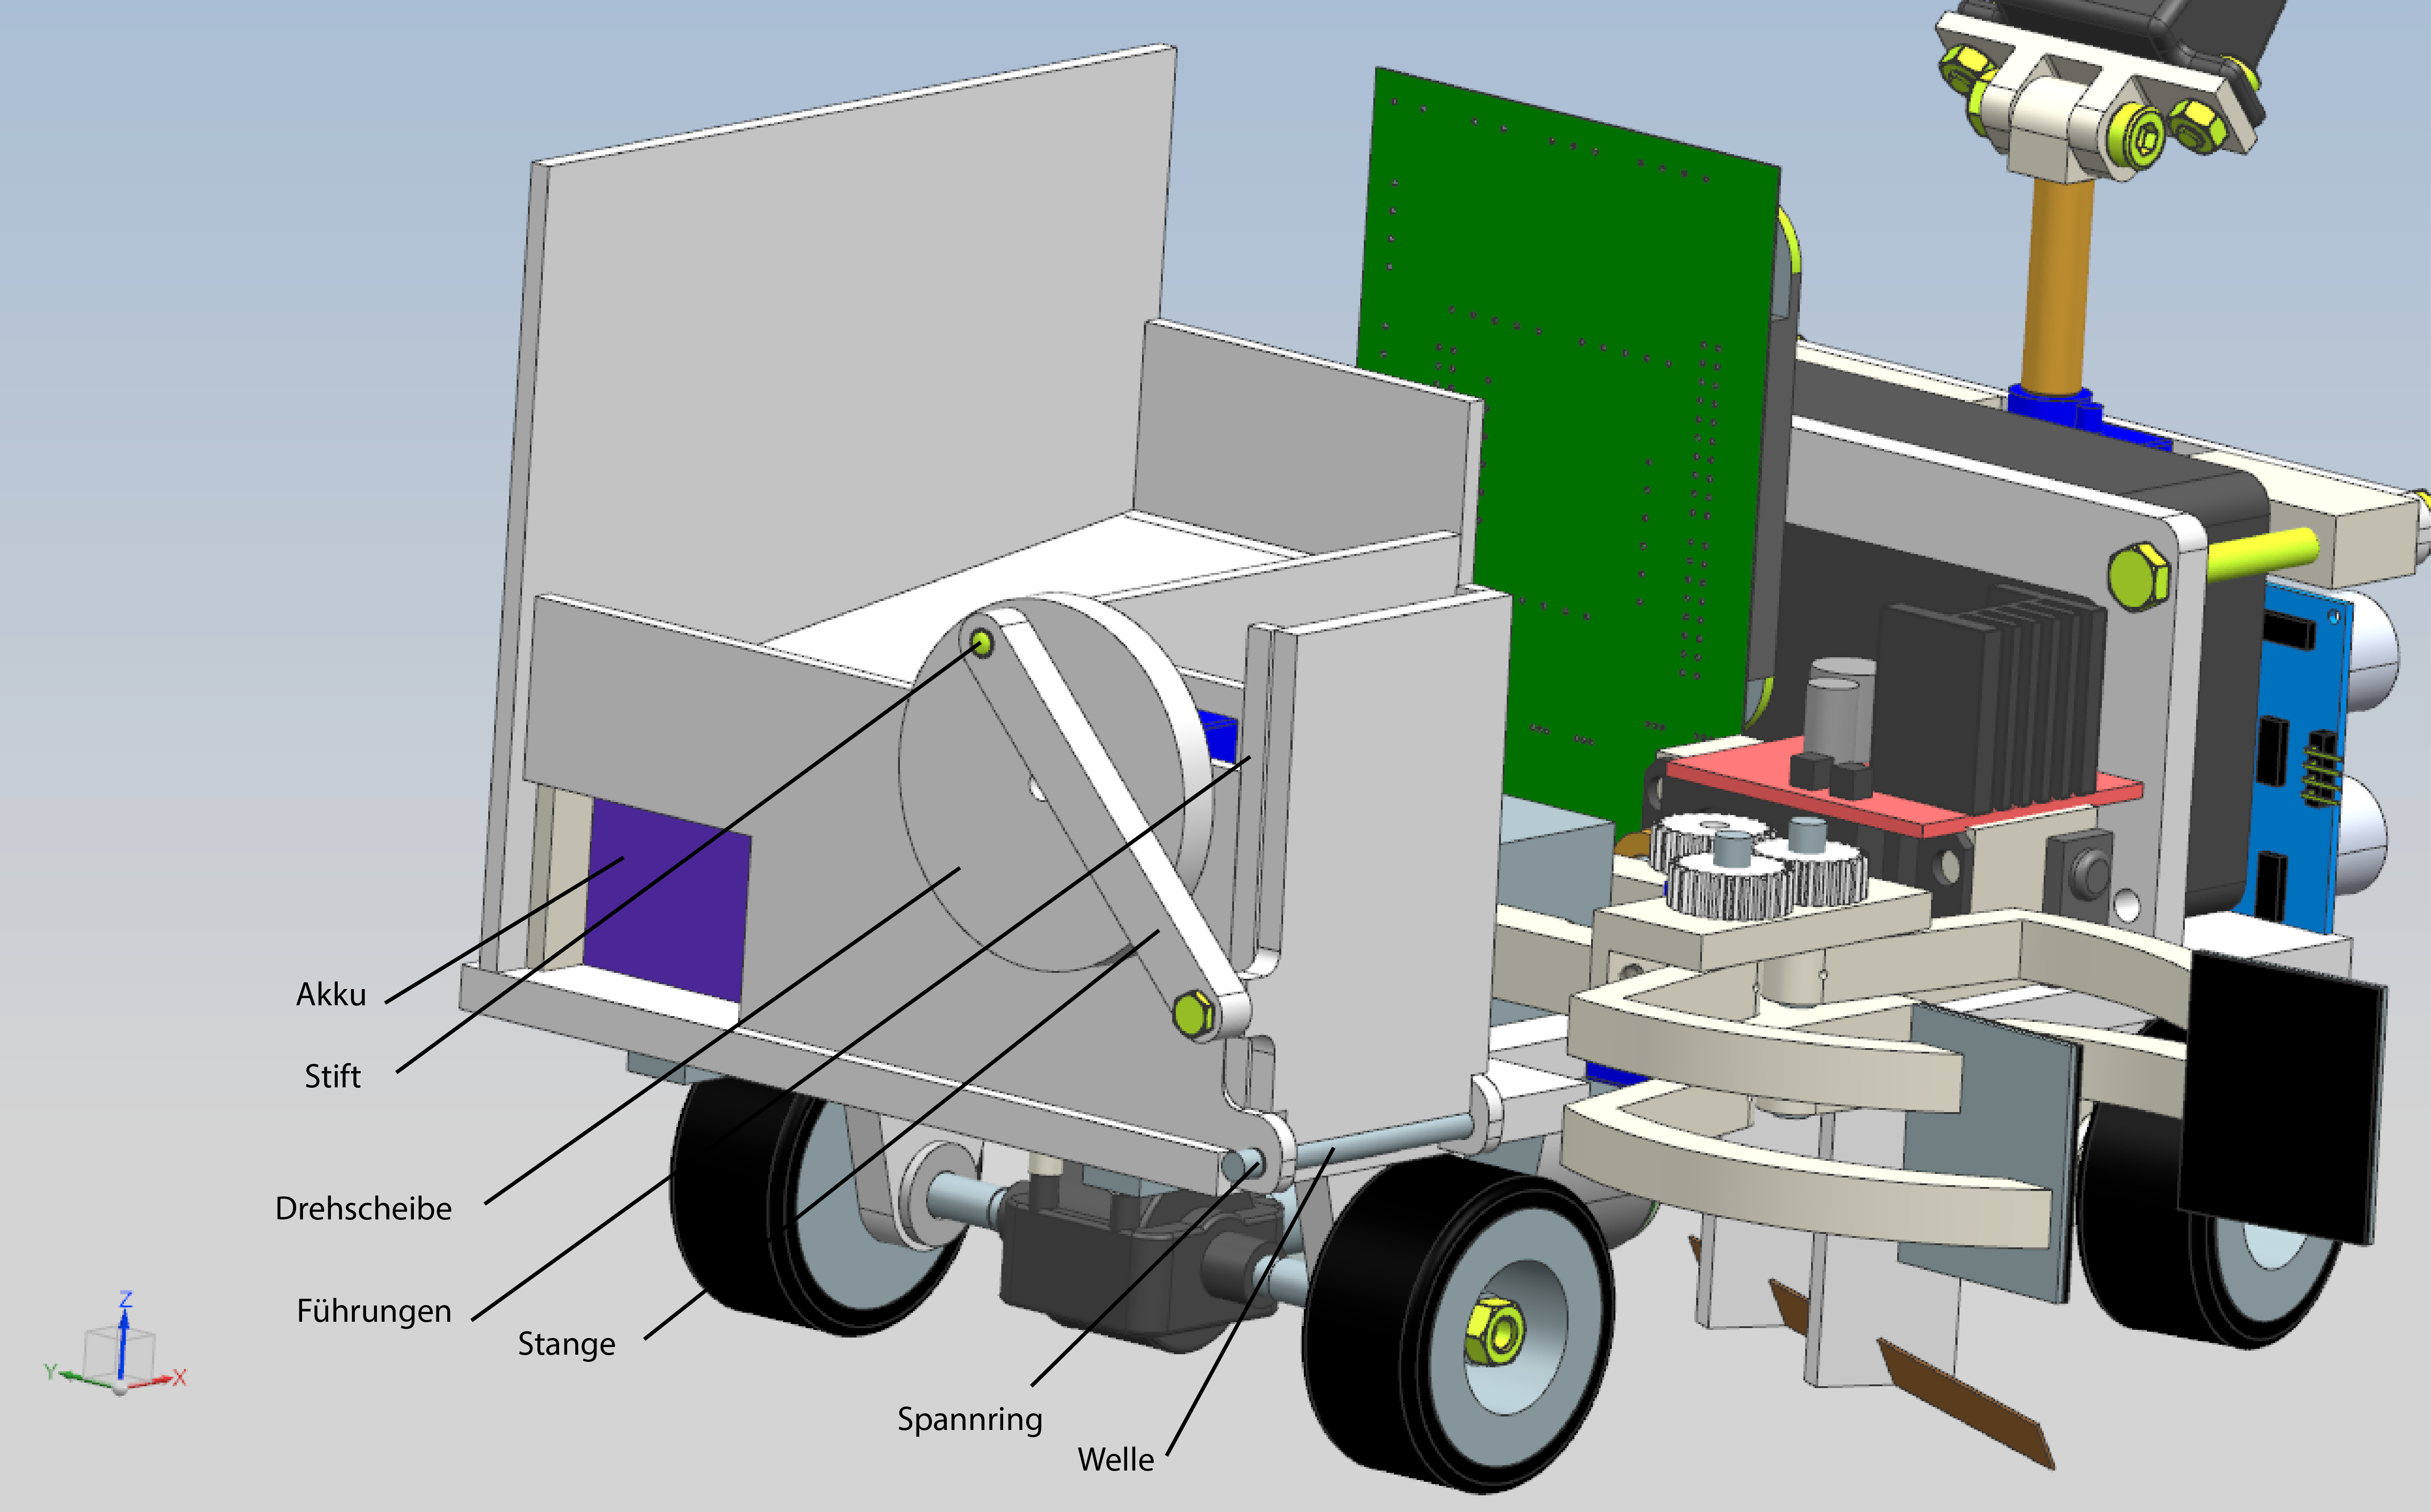
\includegraphics[width=1\textwidth]{03_Loesungskonzept/pictures/entladen12.png}
\caption{Entladen}
\end{figure}
Beim Entladevorgang fährt das Fahrzeug bis Mitte des Entladebehälter. Anschliessend wird die Klappe geöffnet. Über die Klappe rutscht das Schüttgut in das Entsorgungsbecken. Nach erfolgter Abladung wird die Klappe wieder nach oben gezogen und ist wieder in der Ausgangsstellung.\\[0.2cm]
Der Servo Motor wird auf der linken Behälterwand montiert. Auf dem Motor ist die Drehscheibe (Acrylglas) befestigt. Nahe des Randes wurde ein Stift eingesetzt, der die Verbindung zur Stange herstellt. Die Stange wurde an der Entladeklappe (Laserschneideteil Acrylglas) verschraubt.
An den Behälterwänden links und rechts der Gleitfläche sind Bohrungen für die Welle angebracht. Diese wurde mit Spannringen befestigt. Auf der Welle und auf der Entladeklappe sind Schlitze angebracht damit diese über ein Blech und Kleber verbunden werden können.
Auf der Entladeklappe sind rechts und links Führungen (Laserschneidteile) angebracht um der Schraubenfluss zu lenken und bei geschlossener Klappe zu verhindern, dass Schrauben frühzeitig herausfallen.\\[0.2cm]
\\
\textbf{Vergleich Konzept und Umsetzung}\\[0.2cm]
Das Öffnen bzw. Schliessen der Klappe wird mit einem deutlich einfacheren und schnelleren Mechanismus bewerkstelligt. Die Klappe wird mit einem Drehscheibe-Stangen Mechanismus bewegt.\\[0.2cm]